\documentclass[aspectratio=169]{beamer}
\usetheme{boxes}
\usepackage{bm}
\usepackage{booktabs}
\usepackage{amsfonts}
\usepackage{amssymb}
\usepackage{amsmath}
\usepackage{amsthm}
\usepackage{comment}
\usepackage{geometry}
% Removed algorithmic packages to avoid conflicts
\usepackage{graphicx}
\usepackage{hyperref}
\usepackage{subcaption}
\usepackage{tikz}
% \usepackage{physics} % Removed due to conflicts with essay-def
\usepackage{xcolor}
\usepackage{listings}
\usepackage{essay-def}
% Configure itemize for beamer
\newcommand{\JX}[1]{{\color{blue}{$^{\text{JX}}$[#1]}}}
\setbeamertemplate{itemize item}{\textbullet}
\setbeamertemplate{itemize subitem}{--}
\setbeamertemplate{itemize subsubitem}{*}
\usepackage[version=4]{mhchem}
\geometry{left=1cm,right=1cm}

% Define custom colors matching ByteDance style
\definecolor{highlight}{RGB}{220, 20, 60}
\definecolor{codegreen}{RGB}{0, 128, 0}
\definecolor{codepurple}{RGB}{128, 0, 128}

% Define styled hyperlink command
\newcommand{\styhref}[2]{\href{#1}{\textcolor{highlight}{\underline{#2}}}}

% Code listing style
\lstset{
  basicstyle=\ttfamily\footnotesize,
  keywordstyle=\color{blue},
  commentstyle=\color{codegreen},
  stringstyle=\color{codepurple},
  breaklines=true,
  frame=single,
  backgroundcolor=\color{gray!5},
  showspaces=false,
  showstringspaces=false,
  showtabs=false,
  tabsize=4,
  keepspaces=true,
  columns=flexible,
  xleftmargin=0pt,
  xrightmargin=0pt
}

\title[AI Agents]{AI Agents Review}
\subtitle{21 Days with Claude Code}
\author[J. Zhao \& CC]{Zhao Jiaxi (NUS) \& Claude Code (Anthropic)}
\date[\today]{\today}

\begin{document}

\begin{frame}
\titlepage
\end{frame}

\begin{frame}{Outline}
\tableofcontents
\end{frame}

% ==========================
% Section 1: What is Agent and Why Agent? (6 pages)
% ==========================
\section{What is Agent and Why Agent?}

\begin{frame}
	\begin{center}
		\Large
		\textbf{What is Agent and Why Agent?}
	\end{center}
\end{frame}

\begin{frame}{What is an Agent?}
	% TODO: this slide is a bit wordy
	\begin{block}{Formal Definition (Russell \& Norvig)}
		"An agent is anything that perceives its \textbf{environment} through sensors and acts upon that environment through \textbf{actuators}."
	\end{block}
	
	\vspace{0.3cm}
	
	\begin{columns}
		\column{0.5\textwidth}
		\textbf{Key Characteristics:}
		\begin{itemize}
			\item {\color{highlight}Autonomy}: Acts independently
			\item {\color{highlight}Perception}: Senses environment
			\item {\color{highlight}Action}: Changes environment
			\item {\color{highlight}Goal-directed}: Works toward objectives
		\end{itemize}
		
		\column{0.5\textwidth}
		\textbf{In AI Context:}
		\begin{itemize}
			\item Software that performs tasks with minimal supervision
			\item Makes decisions to maximize goals
			\item Can learn and adapt over time
			\item Ranges from thermostats to LLMs
		\end{itemize}
	\end{columns}
	
	\vspace{0.3cm}
	
	\begin{center}
		\small
		{\color{gray}Etymology: From Latin \textit{agere} (to do) - "action on behalf of"}
	\end{center}
\end{frame}

\begin{frame}{Tool Use: Signal of Early Intelligence}
	\begin{columns}
		\column{\textwidth}
		\begin{itemize}
			\item {\color{highlight}Anthropological perspective}: Tool use marks cognitive revolution
			\begin{itemize}
				\item Stone tools $\rightarrow$ Agriculture $\rightarrow$ Writing systems
				\item Cognitive leap: from reactive to proactive behavior
			\end{itemize}
			\item {\color{highlight}AI parallel}: From language generation to action
			\begin{itemize}
				\item GPT-3 (2020): Pure text generation
				\item WebGPT (2021): Web browsing capability
				\item ChatGPT Plugins (2023): Third-party tool ecosystem
				\item Claude Code (2025): Full IDE integration
			\end{itemize}
		\end{itemize}
	\end{columns}
\end{frame}

\begin{frame}{Eliminating Hallucination Through Grounding}
	\begin{itemize}
		\item {\color{highlight}Problem}: LLMs generate plausible but incorrect information
		\item {\color{highlight}Solution}: Ground responses in external tools and data
	\end{itemize}
	
	\begin{columns}
		\column{0.5\textwidth}
		\begin{block}{Without Tools}
			\small
			\texttt{Q: What is sqrt(144)?} \\
			\texttt{A: sqrt(144) = 13} \\
			{\color{red}$\times$ Hallucination}
		\end{block}
		
		\column{0.5\textwidth}
		\begin{block}{With Calculator Tool}
			\small
			\texttt{Thought: Use calculator} \\
			\texttt{Action: calc(sqrt(144))} \\
			\texttt{Result: 12} \\
			\texttt{A: sqrt(144) = 12} \\
			{\color{green}$\checkmark$ Grounded}
		\end{block}
	\end{columns}
	
	\vspace{0.5cm}
	
	\begin{center}
		\textbf{Key Insight:} Grounding in external tools eliminates hallucination
	\end{center}
\end{frame}

\begin{frame}{Environmental Interaction Paradigm}
	\begin{center}
		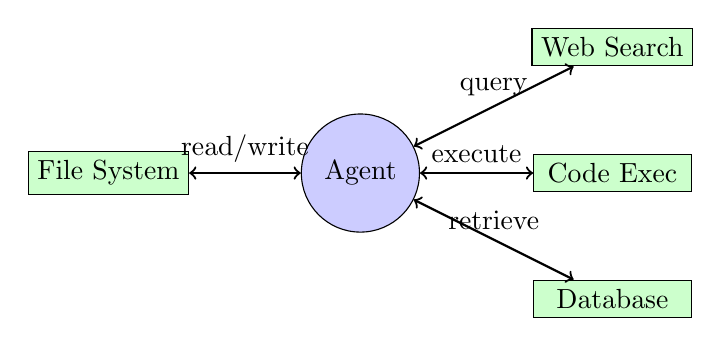
\begin{tikzpicture}[scale=0.8]
			% Agent
			\node[circle, draw, fill=blue!20, minimum size=1.5cm] (agent) at (0,0) {Agent};
			
			% Environment components
			\node[rectangle, draw, fill=green!20, minimum width=2cm] (web) at (4,2) {Web Search};
			\node[rectangle, draw, fill=green!20, minimum width=2cm] (code) at (4,0) {Code Exec};
			\node[rectangle, draw, fill=green!20, minimum width=2cm] (db) at (4,-2) {Database};
			\node[rectangle, draw, fill=green!20, minimum width=2cm] (file) at (-4,0) {File System};
			
			% Arrows
			\draw[<->, thick] (agent) -- (web) node[midway, above] {query};
			\draw[<->, thick] (agent) -- (code) node[midway, above] {execute};
			\draw[<->, thick] (agent) -- (db) node[midway, above] {retrieve};
			\draw[<->, thick] (agent) -- (file) node[midway, above] {read/write};
		\end{tikzpicture}
	\end{center}
	
	\begin{itemize}
		\item {\color{highlight}Perception}: Read from environment (search, query, read)
		\item {\color{highlight}Action}: Modify environment (write, execute, call)
		\item {\color{highlight}Learning}: Adapt based on feedback
	\end{itemize}
\end{frame}

% TEMP COMMENTED OUT FOR DEBUGGING
%\begin{frame}{Agent-Environment Interaction: RL Framework}
%	\begin{center}
%		\begin{tikzpicture}[scale=0.8]
%			% Agent
%			\node[rectangle, draw, fill=blue!30, minimum width=2.5cm, minimum height=1cm] (agent) at (0,0) {Agent (LLM)};
%			
%			% Environment
%			\node[rectangle, draw, fill=green!30, minimum width=3cm, minimum height=1.5cm] (env) at (6,0) {Environment\\Tools, APIs, Files};
%			
%			% State arrow
%			\draw[->, thick, red] (env) to[bend left=30] (agent) node[midway, above] {State $s_t$};
%			
%			% Action arrow  
%			\draw[->, thick, blue] (agent) to[bend left=30] (env) node[midway, below] {Action $a_t$};
%			
%			% Reward arrow
%			\draw[->, thick, purple] (env) to[bend left=60] (agent) node[midway, above left] {Reward $r_t$};
%		\end{tikzpicture}
%	\end{center}
%	
%	\vspace{0.3cm}
%	
%	\begin{columns}
%		\column{0.5\textwidth}
%		\textbf{RL Components:}
%		\begin{itemize}
%			\item {\color{red}State}: Context + tool outputs
%			\item {\color{blue}Action}: Tool calls + text generation  
%			\item {\color{purple}Reward}: Task success + human feedback
%		\end{itemize}
%		
%		\column{0.5\textwidth}
%		\textbf{Evolution via RL:}
%		\begin{itemize}
%			\item Learn which tools to use when
%			\item Improve reasoning strategies
%			\item Adapt to user preferences
%		\end{itemize}
%	\end{columns}
%	
%	\vspace{0.3cm}
%	\begin{center}
%		{\color{highlight}Agents can improve through environmental interaction}
%	\end{center}
%\end{frame}

\begin{frame}{Agent Learning Through Environment}
	\textbf{Key Concept:} Agents can evolve and improve through reinforcement learning
	
	\vspace{0.5cm}
	
	\begin{itemize}
		\item {\color{highlight}State}: Current context + tool outputs
		\item {\color{highlight}Action}: Tool calls + text generation
		\item {\color{highlight}Reward}: Task success + human feedback
	\end{itemize}
	
	\vspace{0.5cm}
	
	\textbf{Learning Goals:}
	\begin{itemize}
		\item Learn optimal tool selection
		\item Improve reasoning strategies  
		\item Adapt to user preferences
	\end{itemize}
\end{frame}

\begin{frame}{Evolution: From Prompting to Agents}
	\begin{center}
		\begin{tabular}{|l|c|c|c|c|}
			\hline
			\textbf{Capability} & \textbf{Prompting} & \textbf{Tool Use} & \textbf{Agents} & \textbf{Advanced} \\
			\hline
			User Control & High & Medium & Low & Guided \\
			Context Length & Limited & Limited & Extended & Extended* \\
			Error Recovery & Manual & Manual & Semi-auto & Semi-auto \\
			Task Complexity & Simple & Medium & Complex & Complex \\
			\hline
			\textbf{Example} & ChatGPT & Plugins & Claude Code & ??? \\
			\hline
		\end{tabular}
	\end{center}
	
	\vspace{0.5cm}
	
	\begin{itemize}
		\item {\color{highlight}Prompting Era} (2020-2022): Chain-of-thought, few-shot learning
		\item {\color{highlight}Tool Use Era} (2022-2024): Function calling, structured outputs
		\item {\color{highlight}Early Agent Era} (2024-2025): Planning, memory, basic workflows
		\item {\color{highlight}Future} (2025+): Enhanced reliability, domain specialization
	\end{itemize}
	
\end{frame}

% ==========================
% Section 2: How to Build Agent? (5 pages)
% ==========================
\section{How to Build Agent?}

\begin{frame}
	\begin{center}
		\Large
		\textbf{How to Build Agent?}

	\end{center}
\end{frame}

\begin{frame}[fragile]{Tool Use Mechanism: System prompts v.s. Function calling}
	\begin{block}{Pattern Recognition for Tool Calls}
		LLMs output text $\rightarrow$ System recognizes patterns $\rightarrow$ Triggers tool execution
	\end{block}

		\textbf{OpenAI Function Calling:}
\begin{lstlisting}
{
  "role": "assistant",
  "content": null,
  "function_call": {
    "name": "get_weather",
    "arguments": "{\"location\": \"SF\"}"
  }
}
\end{lstlisting}
	
	\vspace{0.3cm}
	\begin{itemize}
		\item {\color{highlight}JSON Schema}: Structured output for reliable parsing (Claude's tool use format)
		\item {\color{highlight}XML Tags}: Better prompt readability and flexibility
	\end{itemize}
\end{frame}

\begin{frame}[fragile]{MCP: Model Context Protocol}
		\begin{itemize}
			\item {\color{highlight}Standardized protocol} for LLM-tool communication that separates tools from AI agents
			\item {\color{highlight}Key Components}:
			\begin{itemize}
				\item MCP server (calls tools), agent (MCP client)
				\item Tool registration and discovery
				\item Execution sandbox
				\item Result formatting
			\end{itemize}
			\item {\color{highlight}Benefits}:
			\begin{itemize}
				\item Tool interoperability
				\item Security isolation
				\item Consistent interfaces
			\end{itemize}
			\item More info: \styhref{https://www.bilibili.com/video/BV1aeLqzUE6L/?spm_id_from=333.337.search-card.all.click&vd_source=33f55e2440bef2f106246ccd65bf1daed}{Bilibili Video}
		\end{itemize}

\end{frame}

\begin{frame}{Agentic Workflows}
	\begin{center}
		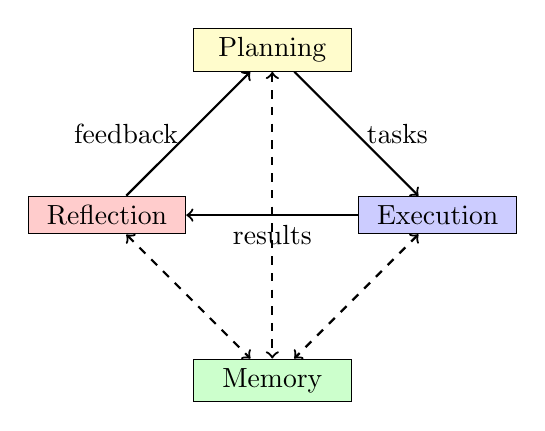
\begin{tikzpicture}[scale=0.7]
			% Planning
			\node[rectangle, draw, fill=yellow!20, minimum width=2cm] (plan) at (0,3) {Planning};
			
			% Execution
			\node[rectangle, draw, fill=blue!20, minimum width=2cm] (exec) at (3,0) {Execution};
			
			% Reflection
			\node[rectangle, draw, fill=red!20, minimum width=2cm] (reflect) at (-3,0) {Reflection};
			
			% Memory
			\node[rectangle, draw, fill=green!20, minimum width=2cm] (memory) at (0,-3) {Memory};
			
			% Arrows
			\draw[->, thick] (plan) -- (exec) node[midway, right] {tasks};
			\draw[->, thick] (exec) -- (reflect) node[midway, below] {results};
			\draw[->, thick] (reflect) -- (plan) node[midway, left] {feedback};
			
			\draw[<->, thick, dashed] (plan) -- (memory);
			\draw[<->, thick, dashed] (exec) -- (memory);
			\draw[<->, thick, dashed] (reflect) -- (memory);
		\end{tikzpicture}
	\end{center}
	
	\begin{columns}
		\column{0.5\textwidth}
		\begin{itemize}
			\item {\color{highlight}Planning}: Task decomposition
			\item {\color{highlight}Execution}: Tool calls, actions
		\end{itemize}
		
		\column{0.5\textwidth}
		\begin{itemize}
			\item {\color{highlight}Reflection}: Self-critique
			\item {\color{highlight}Memory}: Context persistence
		\end{itemize}
	\end{columns}
\end{frame}

\begin{frame}{Training Agents: Beyond Pre-training}
	\begin{tabular}{|l|p{3cm}|p{3cm}|p{3cm}|}
		\hline
		\textbf{Stage} & \textbf{Pre-training} & \textbf{Fine-tuning} & \textbf{Agent Training} \\
		\hline
		\textbf{Objective} & Next token prediction & Task-specific & Tool use + Planning \\
		\hline
		\textbf{Data} & Web text & Labeled examples & Trajectories \\
		\hline
		\textbf{Scale} & Trillions of tokens & Thousands & Millions of steps \\
		\hline
		\textbf{Method} & Self-supervised & Supervised & IL/RL/Self-play \\
		\hline
	\end{tabular}
	
	\vspace{0.5cm}
	
	\begin{itemize}
		\item {\color{highlight}Imitation Learning}: Learn from human demonstrations
		\begin{itemize}
			\item WebGPT: 6K demonstrations of web browsing
		\end{itemize}
		\item {\color{highlight}Reinforcement Learning}: Optimize for task rewards
		\begin{itemize}
			\item RLHF for preference alignment
		\end{itemize}
		\item {\color{highlight}Self-improvement}: Generate and learn from own data
		\begin{itemize}
			\item Toolformer: Self-supervised API call insertion
		\end{itemize}
	\end{itemize}
\end{frame}

\begin{frame}[fragile]{Agent Frameworks: LangChain \& LangGraph}
	\begin{columns}
		\column{0.5\textwidth}
		\textbf{LangChain:}
		\begin{itemize}
			\item Chain-based architecture
			\item Sequential, linear workflows
			\item High-level abstractions
		\end{itemize}
		\begin{lstlisting}[language=python]
from langchain.chains import LLMChain
from langchain.llms import OpenAI

chain = LLMChain(
    llm=OpenAI(),
    prompt=prompt_template,
    memory=ConversationBufferMemory()
)
result = chain.run(query)
\end{lstlisting}
		
		\column{0.5\textwidth}
		\textbf{LangGraph:}
		\begin{itemize}
			\item Graph-based with cycles
			\item Stateful, complex workflows
			\item Low-level control
		\end{itemize}
		\begin{lstlisting}[language=python]
from langgraph.graph import StateGraph

workflow = StateGraph(state_schema)
workflow.add_node("plan", planning_node)
workflow.add_node("act", action_node)
workflow.add_edge("plan", "act")
workflow.add_conditional_edges("act", should_continue)
app = workflow.compile()
\end{lstlisting}
	\end{columns}
\end{frame}

% ==========================
% Section 3: Agent Literature Review (5 pages)
% ==========================
\section{Agent Literature Review}

\begin{frame}
	\begin{center}
		\Large
		\textbf{Agent Literature Review}
	\end{center}
\end{frame}

\begin{frame}{WebGPT: First Large-Scale Web-Browsing LLM}
		
		\begin{itemize}
			\item Text-based browser environment
			\item Imitation learning from humans: 6K human demonstrations
			\item RLHF for alignment: 20K preference comparisons
			\item Performing rejection sampling against a reward model:
			{\color{highlight}56\%} preferred over humans, {\color{highlight}69\%} vs Reddit answers
		\item Provides factual answers with citations
		\end{itemize}
	\begin{figure}
		\includegraphics[width=0.7\textwidth]{fig/WebGPT.jpg}
	\end{figure}
	\footnotetext[1]{\footnotesize Nakano, Reiichiro, et al. "WebGPT: Browser-assisted question-answering with human feedback." arXiv preprint arXiv:2112.09332, OpenAI, December 2021.}
\end{frame}


\begin{frame}{Toolformer: Self-Supervised Tool Learning}
	\textbf{Self-Supervised Training:}
		\begin{itemize}
			\item[•] {\color{highlight}Step 1:} Sample potential API call positions
			\item[•] {\color{highlight}Step 2:} Execute calls and compute $L_i^+$, $L_i^-$
			\item[•] {\color{highlight}Step 3:} Filter useful calls: $L_i^+ < L_i^- - \tau$
			\item[•] {\color{highlight}Step 4:} Fine-tune on filtered dataset
		\end{itemize}
	\begin{figure}
		\includegraphics[width=\textwidth]{fig/Toolformer.jpg}
	\end{figure}
\end{frame}


\begin{frame}{Toolformer: Self-Supervised Tool Learning}
	\textbf{Weighted Cross-Entropy Loss:}
	$$L_i(z) = -\sum_{j=i}^{n} w_{j-i} \log P_M(x_j | z, x_{1:j-1})$$
	
	\textbf{Filtering Criterion:}
	\begin{align}
		L_i^+ &= L_i(e(c_i, r_i)) \\
		L_i^- &= \min(L_i(\epsilon), L_i(e(c_i, \epsilon)))
	\end{align}
	
	\textit{Where:} $c_i$ = API call, $r_i$ = response, $e(\cdot)$ = embedding
		
	\textbf{Key Insight:}
		API calls are kept only if they {\color{highlight}reduce prediction loss} for future tokens

		\textbf{Limitations:}
	\begin{itemize}
		\item Cannot learn tool usage in chains
	\end{itemize}

	\vspace{0.2cm}
	\footnotetext[2]{\footnotesize Schick, Timo, et al. "Toolformer: Language Models Can Teach Themselves to Use Tools." arXiv preprint arXiv:2302.04761, Meta AI, February 2023.}
\end{frame}


% \begin{frame}[fragile]{MemGPT: Virtual Context Management}
% 	\begin{columns}
% 		\column{0.5\textwidth}
% 		\textbf{OS-Inspired Memory Hierarchy:}
% 		\begin{itemize}
% 			\item {\color{highlight}Main context}: Active working memory
% 			\item {\color{highlight}External storage}: Unlimited capacity
% 			\item {\color{highlight}Paging}: Move data between tiers
% 		\end{itemize}
		
% 		\begin{block}{Memory Operations}
% 			\footnotesize
% 			\begin{lstlisting}
% # Page fault - need external data
% if not in_context(info):
%     page = load_from_storage(info)
%     evict_lru_page()
%     add_to_context(page)
% \end{lstlisting}
% 		\end{block}
		
% 		\column{0.5\textwidth}
% 		\begin{center}
% 			\begin{tikzpicture}[scale=0.6]
% 				\node[rectangle, draw, fill=red!20] (ctx) at (0,2) {Context (8K)};
% 				\node[rectangle, draw, fill=yellow!20] (cache) at (0,0) {Cache (100K)};
% 				\node[rectangle, draw, fill=green!20] (disk) at (0,-2) {Storage ($\infty$)};
				
% 				\draw[<->, thick] (ctx) -- (cache);
% 				\draw[<->, thick] (cache) -- (disk);
% 			\end{tikzpicture}
% 		\end{center}
		
% 		\textbf{Applications:}
% 		\begin{itemize}
% 			\item Document analysis beyond context
% 			\item Multi-session conversations
% 			\item Persistent agent memory
% 		\end{itemize}
% 	\end{columns}
	
% 	\vspace{0.3cm}
% 	\footnotetext[3]{\footnotesize Packer, Charles, et al. "MemGPT: Towards LLMs as Operating Systems." arXiv preprint arXiv:2310.08560, October 2023.}
% \end{frame}


\begin{frame}{ReAct Framework: Synergizing Reasoning and Acting}
	\begin{columns}
		\column{0.5\textwidth}
		\textbf{Traditional Action-Only Loop:}
		\begin{center}
			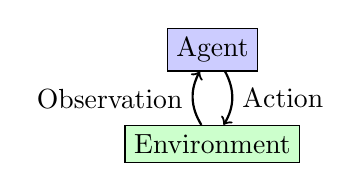
\begin{tikzpicture}[scale=0.6]
				% Simple loop
				\node[rectangle, draw, fill=blue!20] (agent) at (0,2) {Agent};
				\node[rectangle, draw, fill=green!20] (env) at (0,0) {Environment};
				
				\draw[->, thick] (agent) to[bend left=30] node[right] {Action} (env);
				\draw[->, thick] (env) to[bend left=30] node[left] {Observation} (agent);
			\end{tikzpicture}
		\end{center}
		
		\column{0.5\textwidth}
		\textbf{ReAct Framework:}
		\begin{center}
			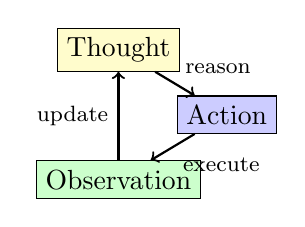
\begin{tikzpicture}[scale=0.55]
				% ReAct cycle
				\node[rectangle, draw, fill=yellow!20] (thought) at (0,3) {Thought};
				\node[rectangle, draw, fill=blue!20] (action) at (2.5,1.5) {Action};
				\node[rectangle, draw, fill=green!20] (obs) at (0,0) {Observation};
				
				\draw[->, thick] (thought) -- (action) node[midway, above right] {\footnotesize reason};
				\draw[->, thick] (action) -- (obs) node[midway, below right] {\footnotesize execute};
				\draw[->, thick] (obs) -- (thought) node[midway, left] {\footnotesize update};
			\end{tikzpicture}
		\end{center}
		
	\end{columns}
	\vspace{0.3cm}
	\textbf{Key Innovation:} Interleaved reasoning traces and actions via few-shot in-context examples
		
		\begin{itemize}
			\item Uses a frozen language model (PaLM-540B) with few-shot in-context examples
			\item Baselines: Standard (w/o reasoning + observation), CoT (w/o observation + action), ACT (w/o reasoning)
		\end{itemize}
	
	\footnotetext[3]{\footnotesize Yao, Shunyu, et al. "ReAct: Synergizing Reasoning and Acting in Language Models." International Conference on Learning Representations (ICLR), 2023.}
\end{frame}

\begin{frame}{ReAct: Example Trace}
		\begin{block}{ReAct Trace Example}
			\footnotesize
			\texttt{Question: What is the elevation of Mt. Everest?}\\
			\texttt{Thought: I need to search for Mt. Everest}\\
			\texttt{Action: search[Mt. Everest]}\\
			\texttt{Observation: Mt. Everest is Earth's highest mountain}\\
			\texttt{Thought: I need the specific elevation}\\
			\texttt{Action: lookup[elevation]}\\
			\texttt{Observation: 8,849 meters (29,032 ft)}\\
			\texttt{Thought: I have the answer}\\
			\texttt{Answer: 8,849 meters}
		\end{block}
		
		\textbf{Results:}
		\begin{itemize}
			\item HotpotQA: {\color{highlight}27\% improvement}, ALFWorld: {\color{highlight}34\% over RL baselines},
			WebShop: {\color{highlight}10\% improvement}
			\item Reduces error propagation in multi-hop QA
		\end{itemize}
\end{frame}



% ==========================
% Section 4: Case Study - Claude Code (15 pages)
% ==========================
\section{Case Study: Claude Code}

\begin{frame}
	\begin{center}
		\Large
		\textbf{Case Study: Claude Code}
	\end{center}
\end{frame}

\begin{frame}[fragile]{Claude Code: Introduction}
		\textbf{What is Claude Code?}
		\begin{itemize}
			\item Anthropic's official CLI for Claude, an AI-powered coding assistant
		\item Released in February 2025
			\item Terminal-based, similar to OpenAI's Codex \& Google's Gemini CLI, different from Cursor and Windsurf
			\item \styhref{https://github.com/anthropics/claude-code}{Source code} available (partially obfuscated)
		\end{itemize}
		
		\textbf{Models Used:}
		\begin{itemize}
			\item Haiku 3.5 (simple tasks, high throughput)
			\item Sonnet 4 (main agent) 
			\item Opus 4.1 (complex tasks)
		\end{itemize}
\end{frame}

\begin{frame}{Architecture: Multi-Agent System}
	\begin{center}
		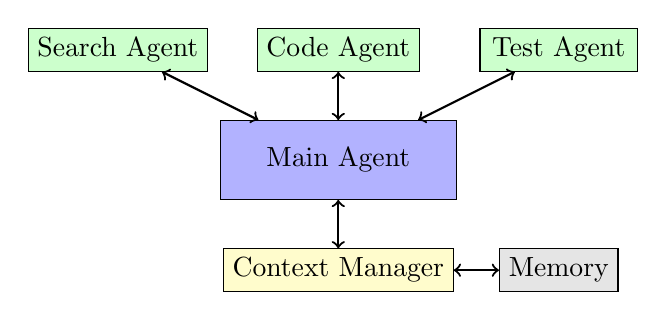
\begin{tikzpicture}[scale=0.7]
			% Main Agent
			\node[rectangle, draw, fill=blue!30, minimum width=3cm, minimum height=1cm] (main) at (0,0) {Main Agent};
			
			% Sub-agents
			\node[rectangle, draw, fill=green!20, minimum width=2cm] (search) at (-4,2) {Search Agent};
			\node[rectangle, draw, fill=green!20, minimum width=2cm] (code) at (0,2) {Code Agent};
			\node[rectangle, draw, fill=green!20, minimum width=2cm] (test) at (4,2) {Test Agent};
			
			% Context Manager
			\node[rectangle, draw, fill=yellow!20, minimum width=2cm] (context) at (0,-2) {Context Manager};
			\node[rectangle, draw, fill=gray!20] (memory) at (4,-2) {Memory};
			
			% Connections
			\draw[<->, thick] (main) -- (search);
			\draw[<->, thick] (main) -- (code);
			\draw[<->, thick] (main) -- (test);
			\draw[<->, thick] (main) -- (context);
			\draw[<->, thick] (context) -- (memory);
		\end{tikzpicture}
	\end{center}
	
	\begin{itemize}
		\item {\color{highlight}Main Agent}: Orchestrates overall task
		\item {\color{highlight}Sub-agents}: Handle specific subtasks in isolation
		\item {\color{highlight}Context Manager}: Optimizes token usage
	\end{itemize}
\end{frame}


\begin{frame}{Reverse Engineering: System Prompts}
	\textbf{Key System Prompt Elements:}
	
	\begin{block}{Core Instructions}
		\footnotesize
		\begin{itemize}
			\item "You are Claude Code, Anthropic's official CLI for Claude"
			\item "Be concise, direct, and to the point"
			\item "Minimize output tokens while maintaining quality"
			\item "Use tools to complete tasks, not for communication"
		\end{itemize}
	\end{block}
	
	\textbf{Behavioral Guidelines:}
	\begin{columns}
		\column{0.5\textwidth}
		\begin{itemize}
			\item Proactive: Use TODO lists
			\item Defensive: Follow conventions
			\item Efficient: Batch operations
		\end{itemize}
		
		\column{0.5\textwidth}
		\begin{itemize}
			\item Safe: Never commit without asking
			\item Clear: Explain complex commands
			\item Adaptive: Learn from context
		\end{itemize}
	\end{columns}
	
	\small
	Source: github.com/Yuyz0112/claude-code-reverse
\end{frame}

\begin{frame}{Agentic Workflow}
	\begin{itemize}
		\item[1.] {\color{highlight}\textbf{Quota Check}} (Haiku 3.5)
		\begin{itemize}
			\item Lightweight API verification
			\item Context initialization
		\end{itemize}
		
		\item[2.] {\color{highlight}\textbf{Task Analysis}} (Main Agent)
		\begin{itemize}
			\item Parse user request
			\item Create TODO list
			\item Plan execution strategy
		\end{itemize}
		
		\item[3.] {\color{highlight}\textbf{Execution Loop}}
		\begin{itemize}
			\item Execute tools in parallel when possible
			\item Update TODO status
			\item Handle errors and retry
		\end{itemize}
		
		\item[4.] {\color{highlight}\textbf{Context Compaction}}
		\begin{itemize}
			\item Isolate "dirty context" in sub-agents
			\item Return only essential results
			\item Maintain conversation history
		\end{itemize}
	\end{itemize}
\end{frame}

\begin{frame}[fragile]{TODO List: How It Works}
	\textbf{Core Mechanism:}
	\begin{itemize}
		\item {\color{highlight}\textbf{Proactive Creation}}: Agent creates TODO list for complex tasks (2+ steps)
		\item {\color{highlight}\textbf{Real-time Updates}}: Status changes as work progresses
		\item {\color{highlight}\textbf{Atomic Operations}}: Each task marked complete immediately upon finish
	\end{itemize}
	
	\begin{columns}
		\column{0.5\textwidth}
		\begin{block}{JSON Structure}
			\footnotesize
			\begin{lstlisting}
{
  "todos": [
    {
      "content": "Fix authentication bug",
      "activeForm": "Fixing authentication bug", 
      "status": "in_progress"
    },
    {
      "content": "Run tests",
      "activeForm": "Running tests",
      "status": "pending"  
    }
  ]
}
\end{lstlisting}
		\end{block}
		
		\column{0.5\textwidth}
		\textbf{Workflow:}
		\begin{itemize}
			\item[1.] User requests complex task
			\item[2.] Agent creates TODO list
			\item[3.] Exactly ONE task "in\_progress" 
			\item[4.] Complete → mark done → start next
			\item[5.] Continue until all complete
		\end{itemize}
	\end{columns}
\end{frame}

\begin{frame}{TODO List: Dynamic Task Management}
	\begin{columns}
		\column{0.5\textwidth}
		\includegraphics[width=\textwidth]{fig/TODO1.jpg}
		
		\column{0.5\textwidth}
		\textbf{Implementation:}
		\begin{itemize}
			\item Stored in \texttt{\~{}/.claude/todos/}
			\item JSON format
			\item Three states:
			\begin{itemize}
				\item \texttt{pending}
				\item \texttt{in\_progress}
				\item \texttt{completed}
			\end{itemize}
		\end{itemize}
		
		\textbf{Benefits:}
		\begin{itemize}
			\item User visibility
			\item Progress tracking
			\item Task decomposition
			\item Error recovery
		\end{itemize}
	\end{columns}
\end{frame}

\begin{frame}{TODO List: Real Example}
	\includegraphics[width=0.8\textwidth]{fig/TODO2.jpg}
	
	\begin{itemize}
		\item {\color{highlight}Automatic creation} when task complexity detected
		\item {\color{highlight}Real-time updates} as work progresses
		\item {\color{highlight}Hierarchical} task breakdown
	\end{itemize}
\end{frame}

\begin{frame}[fragile]{Test Case: Read Scientific Code (99\%)}
	\textbf{Task:} Understand complex numerical package GPAW (electronic structure calculation, 300K+ lines of code)
	
		\begin{itemize}
			\item $\checkmark$ Trace functions and classes without Go to Definition
			\item $\checkmark$ Connect mathematical derivations and code implementation
			\item $\checkmark$ Analyze the implementation efficiency
		\end{itemize}

	\textbf{Advanced task:}
	\begin{itemize}
		\item Ask CC to implement a Poisson solver for radial functions based on multipole expansion
		\item Status: Difficult to verify correctness and design accuracy tests
	\end{itemize}
\end{frame}

\begin{frame}[fragile]{Test Case: Resolve Environment \& Docker error (99\%)}
	\textbf{Task:} Modify Docker configuration
	\begin{itemize}
		\item $\checkmark$ Debug docker error
		\item $\checkmark$ Run CC in a docker container
		\item $\checkmark$ Perfect solution with a few iterations
	\end{itemize}
	
	\begin{figure}
		\includegraphics[width=0.6\textwidth]{fig/docker1.jpg}
	\end{figure}
	\begin{figure}
		\includegraphics[width=0.6\textwidth]{fig/docker2.jpg}
	\end{figure}
\end{frame}

\begin{frame}[fragile]{Test Case: Integration Testing (90\%)}
	\textbf{Task:} Write tests for the invertibility of normalizing flow models

	\begin{itemize}
		\item Normalizing flow implemented via \textit{distrax} with clear interface
		\item Extremely clear instructions
		\item $\checkmark$ Implemented the desired tests but with some code redundancy
		\begin{lstlisting}[language=python]
# Claude generated test
def test_rqs_identity_composition(self):
    """Test that forward * inverse = identity for RQS transformation."""
    # initialization of the NF...

def test_rqs_inverse_forward_composition(self):
    """Test that inverse * forward = identity for RQS transformation."""
    # initialization of the NF...

def test_rqs_jacobian_consistency(self):
    """Test that the Jacobian of the forward mapping is consistent."""
    # initialization of the NF...
\end{lstlisting}
		\item $\checkmark$ Generated several meaningful new test cases
		\item See more in \styhref{https://github.com/jiaxi98/cnf\_ot/commit/c993a744042e0e4e4593c40b24b8b898c1a0688c}{CC test},
		\styhref{https://github.com/jiaxi98/cnf\_ot/commit/064a69bd308613d9c93d34b637a445601387acb4}{refactor test}
	\end{itemize}
	
	{\color{highlight}Key: Clear interface + complete instructions = High success}
\end{frame}

\begin{frame}{Test Case: Debug NS Solver (20\%)}
	\textbf{Task:} Debug hand-written spectral solver for 2D Navier-Stokes
	\begin{itemize}
		\item $\checkmark$ Figure out the incorrect patterns of the temporal
		correlation functions
		\item {\color{red}$\times$} Failed to identify incorrect real-valued FFT (rfft) treatment
		$\Longrightarrow$ Required self-correction based on human feedback
		\item {\color{red}$\times$} Failed to identify incorrect dealiasing treatment
		$\Longrightarrow$ Required self-correction based on human feedback
	\end{itemize}
	\begin{figure}
		\includegraphics[width=0.48\textwidth]{fig/ns.png}
	\end{figure}
\end{frame}

\begin{frame}{Test Case: Hydra + Ray Training Configuration (0\%)}
	\textbf{Task:} Set up Hydra + Ray for multi-run experiments
	\begin{itemize}
		\item Personal codebase with a relative training interface file train\_jax.py
		\item Clear config system that support hydra multi-run experiments
		\item Integrated with Ray for distributed training (1 run per GPU)
		\item {\color{red}$\times$} Generated overly complex configuration files
		\item {\color{red}$\times$} Cannot configure multiple runs with separate GPUs
	\end{itemize}
\end{frame}


\begin{frame}{Performance Summary}
	\begin{center}
		\begin{tabular}{|l|c|p{5cm}|}
			\hline
			\textbf{Task Type} & \textbf{Score} & \textbf{Key Factors} \\
			\hline
			Code Reading & {\color{green}99\%} & Pattern recognition, documentation \\
			Environment Setup & {\color{green}99\%} & Standard practices, clear goals \\
			Integration Testing & {\color{green}90\%} & Clear interfaces, specifications \\
			Complex Debug & {\color{orange}20\%} & Needs domain expertise \\
			Framework Config & {\color{red}0\%} & Limited training data \\
			Novel Algorithms & {\color{red}N/A} & Beyond current capabilities \\
			\hline
		\end{tabular}
	\end{center}
	
	\vspace{0.5cm}
	
	\textbf{Key Takeaway:}
	\begin{center}
		\large
		{\color{highlight}Claude Code is a powerful amplifier for human developers,}\\
		{\color{highlight}not a replacement for domain expertise}
	\end{center}
\end{frame}


\begin{frame}{Claude Code as a Tool for Humans}
	\textbf{Key Insight:} {\color{highlight}Dramatically lowers barriers} for many tasks
	
	\vspace{0.5cm}

	\begin{columns}
		\column{0.5\textwidth}
		\textbf{Before Claude Code:}
		\begin{itemize}
			\item Hours reading documentation
			\item Manual environment setup
			\item Trial-and-error debugging
			\item Context switching overhead
		\end{itemize}
		
		\column{0.5\textwidth}
		\textbf{With Claude Code:}
		\begin{itemize}
			\item Instant codebase understanding
			\item Automated setup scripts
			\item Guided exploration
			\item Maintained context
		\end{itemize}
	\end{columns}
	
	\vspace{0.5cm}
	
	\begin{block}{Best Use Cases}
		\begin{itemize}
			\item {\color{highlight}Learning new repositories}: Navigate unfamiliar codebases
			\item {\color{highlight}Environment setup}: Docker, dependencies, configuration
			\item {\color{highlight}Boilerplate generation}: Tests, documentation, CI/CD
			\item {\color{highlight}Refactoring}: Systematic code improvements
		\end{itemize}
	\end{block}
\end{frame}


\begin{frame}{Personal Thoughts}
		\begin{itemize}
			\item Optimization over the space of orthogonal matrices
			\begin{equation*}
				\begin{aligned}
				\mathbf{X} & \overset{\text{qr}}{\to} \mathbf{Q} \mathbf{R} \rightarrow L(\mathbf{Q}) \qquad (reparametrization trick)	\\
				\mathcal{L}_{\lambda}(\mathbf{X}) & = \mathcal{L}(\mathbf{X}) + \lambda \left\| \mathbf{X}\mathbf{X}^T - \mathbf{I} \right\|_2^2
				\qquad (\text{penalty method})
				\end{aligned}
			\end{equation*}
			\item Neural network training with equivariant constraint: special architecture design
			enforces the equivariance, e.g. e3nn; Penalty method or data augmentation
			\item Desired properties of LLM agents: Predefined workflow for agent system; Prompt engineering
		\end{itemize}

\end{frame}


\begin{frame}{}
	\begin{center}
		\Huge Thank You!
		
		\vspace{1cm}
		
		\Large Questions?
	\end{center}
\end{frame}

\end{document}Context persistence